\vfill
\textit{This chapter discusses the architecture of following modules:}
\begin{itemize}
    \item Transmitter.
    \begin{itemize}
        \item Chaos Generator.
        \item Modulator.
        \item Transmitter Finite State Machine.
    \end{itemize}
    \item Receiver.

\end{itemize}
\vfill


\newpage
In this chapter, we discuss the architecture of the modem, as well as the design choices made. Figure. \ref{fig:full_mod} shows our proposed architecture to implement the modem. Figure. \ref{fig:dmod} shows the demodulator.


% TODO: These should be SVGs.
\begin{figure}[p]
    \label{fig:full_mod}
    \caption{Transmitter Block Diagram}
    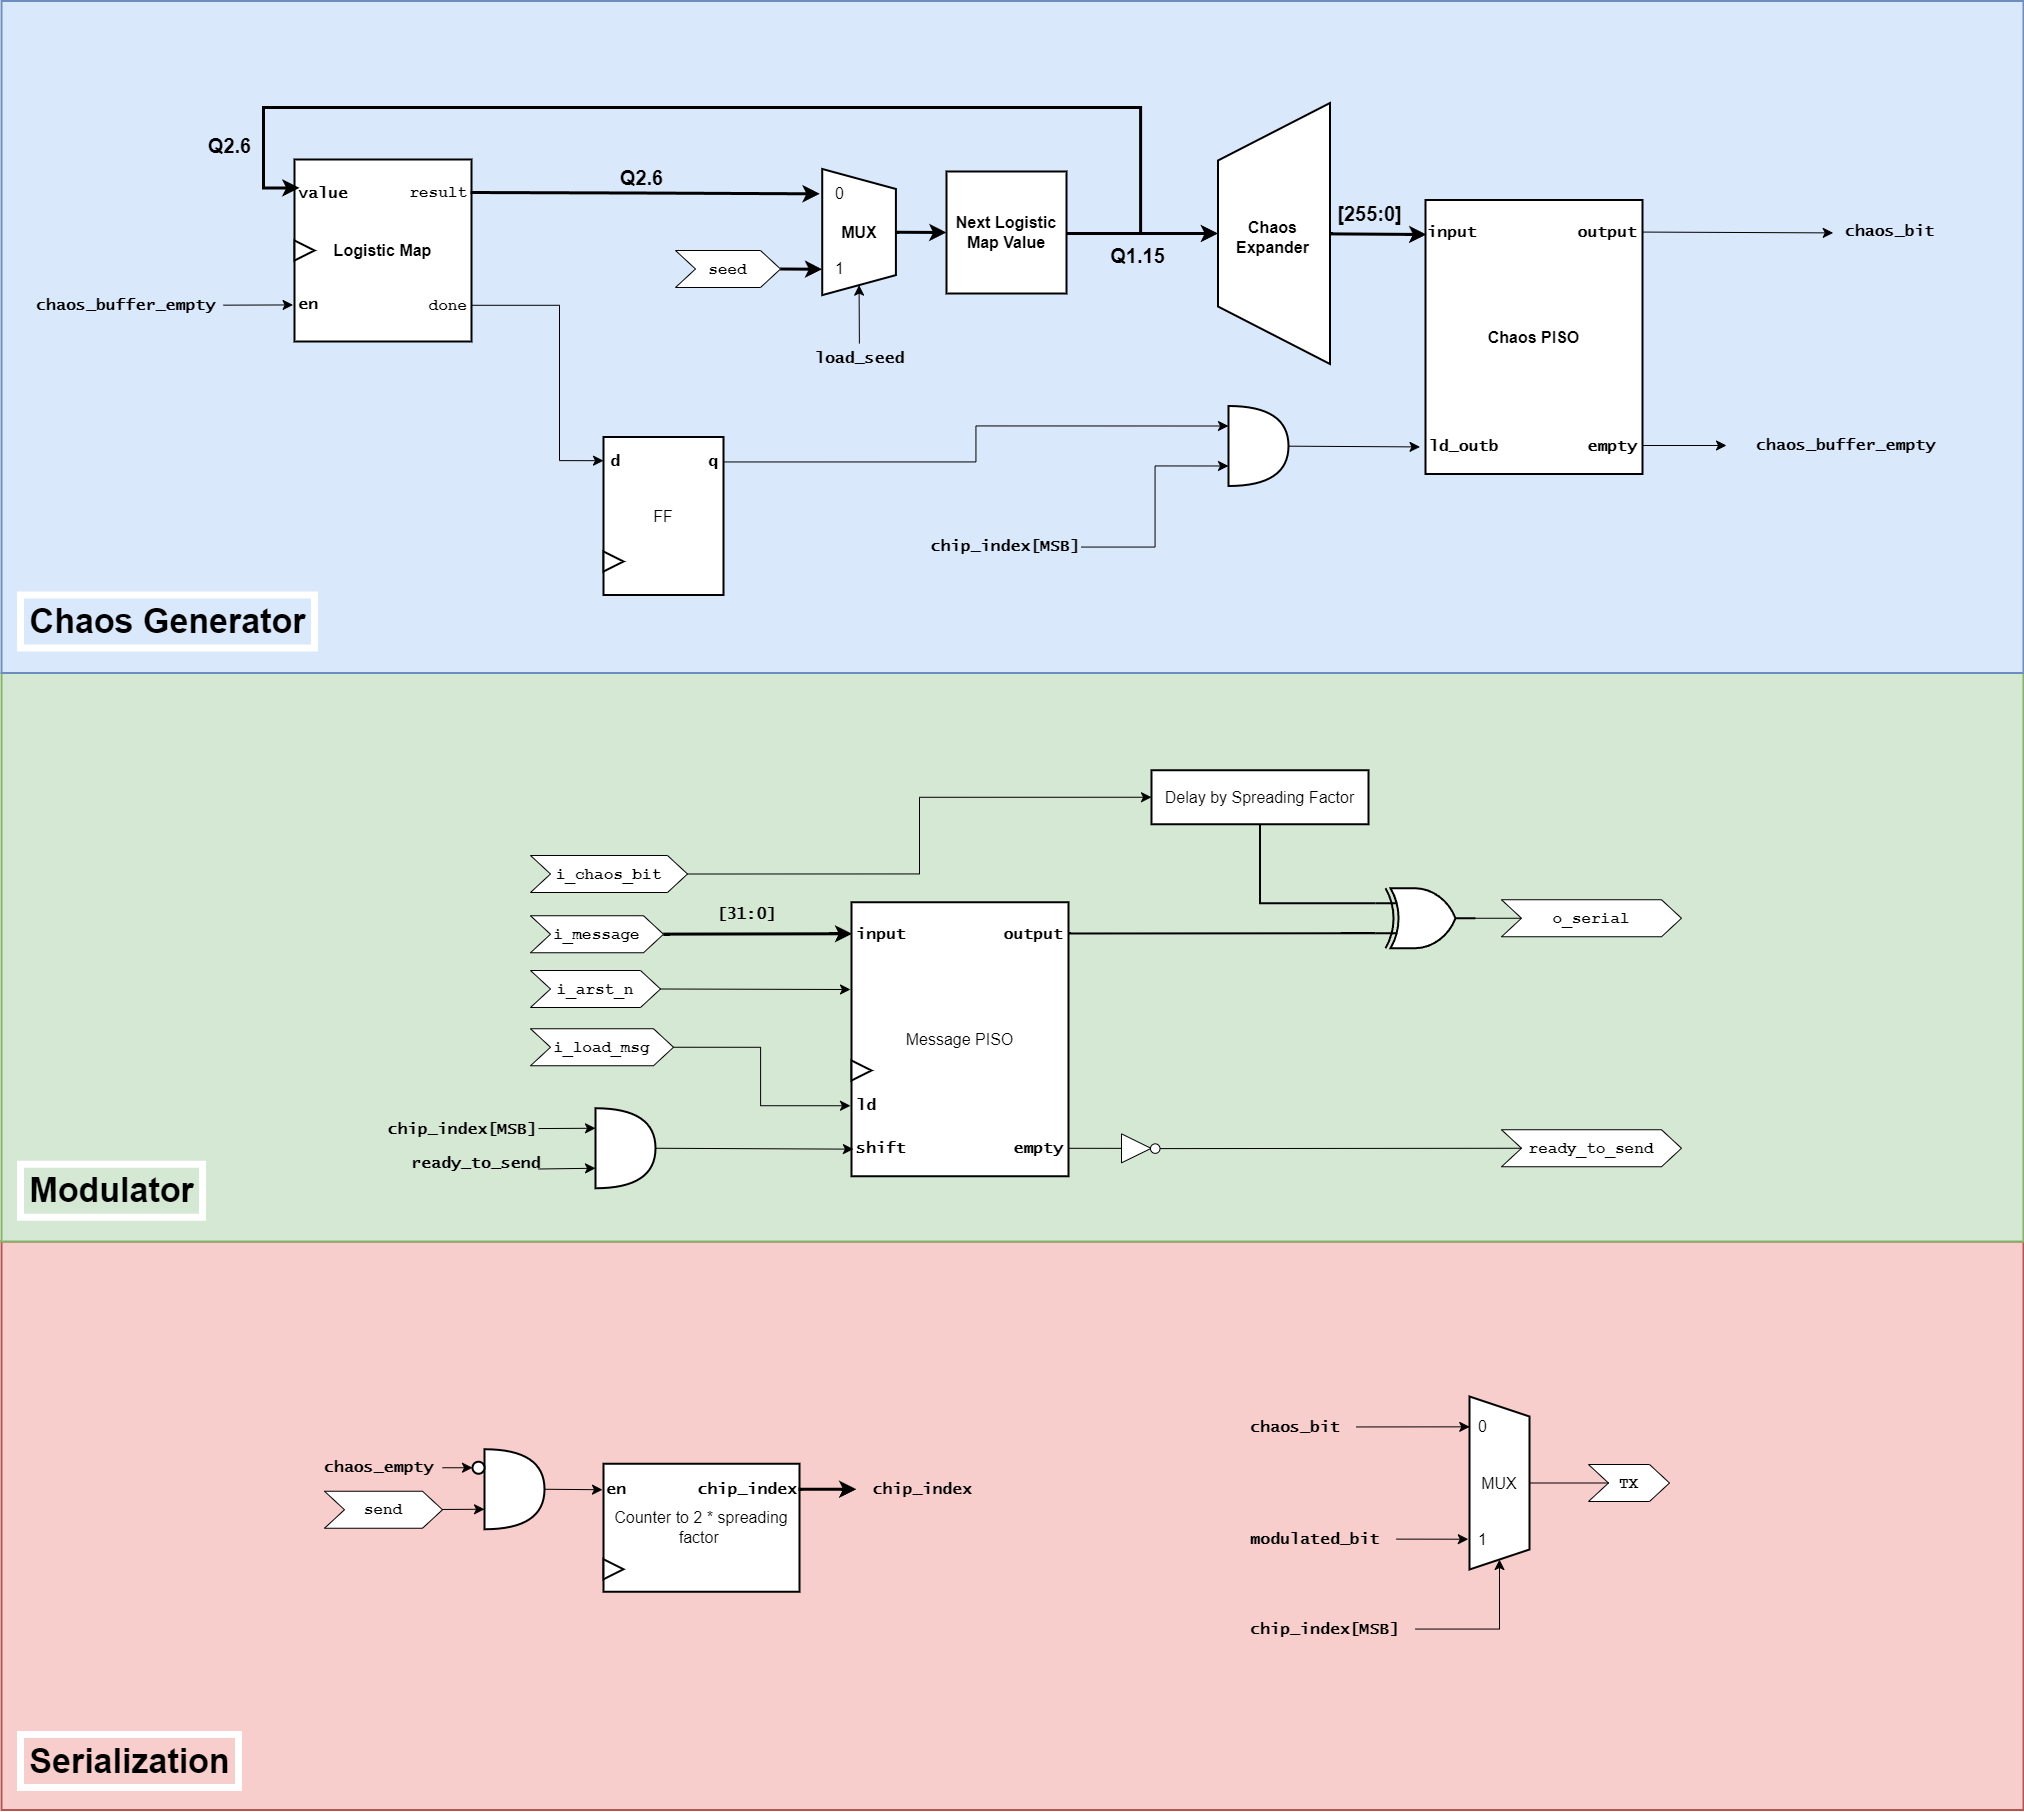
\includegraphics[width=\textwidth]{Top Level/modulator.png}
\end{figure}

\begin{figure}[p]
    \label{fig:dmod}
    \caption{Demodulator Block Diagram}
    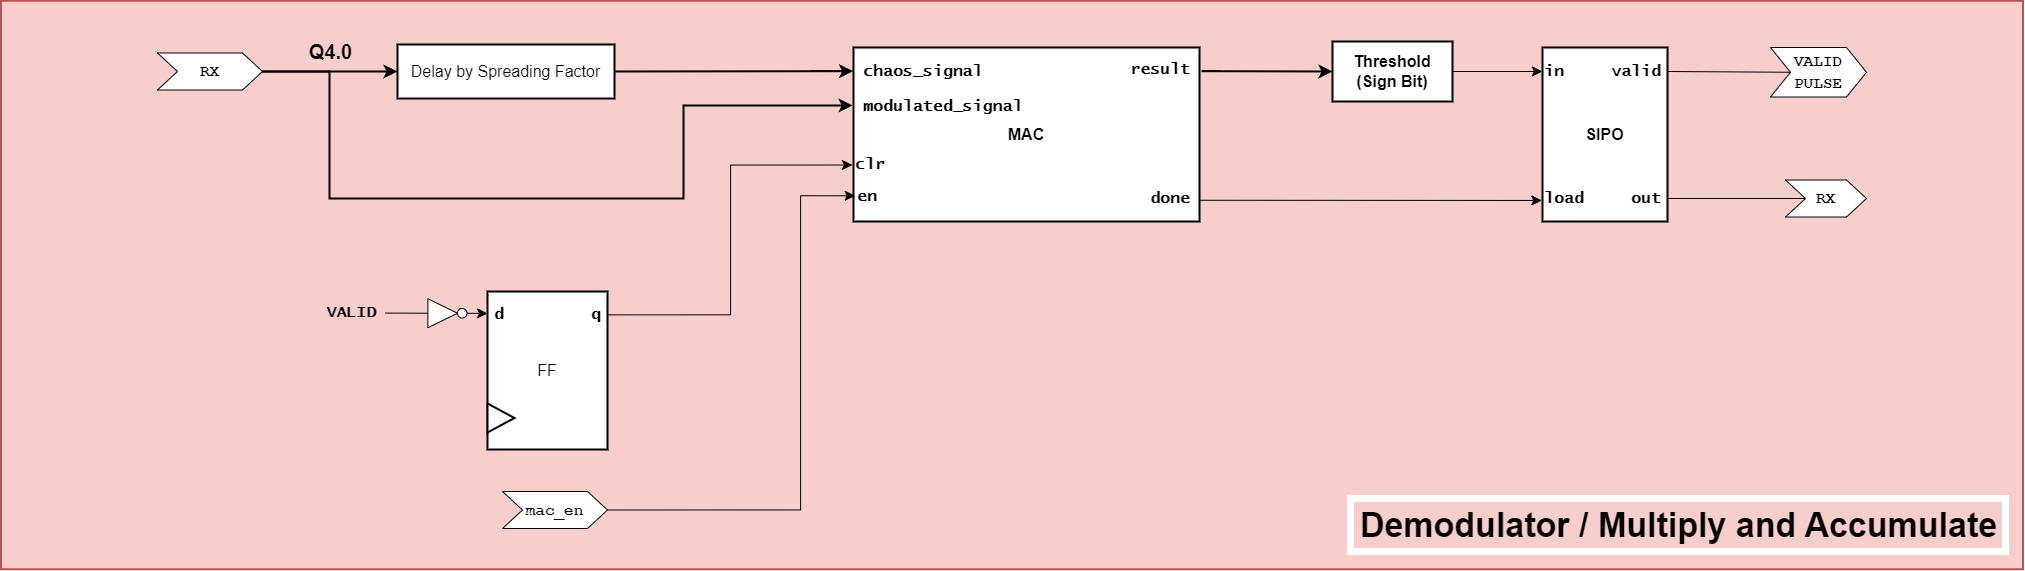
\includegraphics[width=\textwidth]{Top Level/demod.png}
\end{figure}

\section{Transmitter}
The modulator is split into three parts:
\begin{enumerate}
    \item Chaos generator.
    \item Modulator.
    \item Serializer.
\end{enumerate}

\subsection{Chaos Generator}
The chaos is generated with a Logistic Map with $r = 4$. The value $4$ was chosen to simplify the multiplication by $r$ into a shift left by
$2$. The logistic map operates on Q2.6 numbers. From equation \ref{eqn:logistic_map} we can see that if $n_{i}$ is 8-bits in length,
then $n_{i+1}$ is 16-bits. This means that each cycle, the \textsc{Logistic Map} The multiplication is performed with the radix-4 Booth multiplication algorithm. As it
can be seen from the block digaram is shown in Fig.\ref{fig:booth}, all partial products are calculated in parallel meaning that each clock cycle, the module is capable
of generating $16$ bits of chaos.

However, calculating all four partial products in a single sycle each cycle consumes a lot of power. This can happen when the spreading factor is equal to $16$.
Also, 16-bits of chaos is not suffecient for fast data rates.
To solve this, we need to calculate a large number of chaos bits in a short amount of time.
The \textsc{Chaos Expander} takes 16 w y7awel l 256. kamel b2a

\subsection{Modulator}
The purpose of the \textsc{Modulator} is to modulate the chaos bits with the information bits.
The message is first loaded into the \textsc{Message PISO} and is then serially output. The output bit is xor-ed with
a delayed version of the chaos bit from \textsc{Chaos Generator} (delayed by $\beta$).

\begin{center}
    \begin{table}[h]
        \caption{Modulator Pin-Out}
        \vspace*{0.3cm}
    \begin{tabular}{|>{\centering\arraybackslash}m{0.2\textwidth}|>{\centering\arraybackslash}m{0.09\textwidth}|>{\centering\arraybackslash}m{0.1\textwidth}|>{\centering\arraybackslash}m{0.5\textwidth}|}
        \hline
        Name & Width & Direction & Description\\
        \hline
        \texttt{i\_clk} & 1 & Input & Positive edge clock.\\
        \texttt{i\_arst\_n} & 1 & Input & Active-low asynchronous reset.\\
        \texttt{i\_message} & 32 & Input & The input message.\\
        \texttt{i\_chaos\_bit} & 1 & Input & The bit of chaos to be modulated.\\
        \texttt{i\_load\_msg} & 1 & Input & Load the \texttt{Message PISO} with the message at \texttt{i\_message}.\\
        \texttt{o\_ready\_to\_send} & 1 & Output & Asserted if (and only if) the \texttt{Message PISO} is not empty.\\
        \texttt{o\_serial} & 1 & Output & The serial output of the \texttt{Message PISO}.\\
        \hline
    \end{tabular}
    \end{table}
\end{center}

\subsection{Serializer}
This module is the implementation of Equation \ref{eqn:dcsk_frame}. Based on the index of the current chip being sent,
It choses to send the chaos bit, or the modulated bit.
\begin{center}
    \begin{table}[h]
        \caption{Serializer Pin-Out}
        \vspace*{0.3cm}
    \begin{tabular}{|>{\centering\arraybackslash}m{0.2\textwidth}|>{\centering\arraybackslash}m{0.09\textwidth}|>{\centering\arraybackslash}m{0.1\textwidth}|>{\centering\arraybackslash}m{0.5\textwidth}|}
        \hline
        Name & Width & Direction & Description\\
        \hline
        \texttt{i\_clk} & 1 & Input & Positive edge clock.\\
        \texttt{i\_arst\_n} & 1 & Input & Active-low asynchronous reset.\\
        \texttt{i\_chaos\_bit} & 1 & Input & Chaos bit\\
        \texttt{i\_modulated\_bit} & 1 & Input & Modulated bit\\
        \texttt{i\_send} & 1 & Input & A pulse that signals the \textsc{Chip Counter} to start counting.\\
        \texttt{o\_tx} & 1 & Output & Serially output bit.\\
        \hline
    \end{tabular}
    \end{table}
\end{center}

\section{Receiver}
At the heart of the receiver lies the MAC block, which by design, is a correlator. We don't care about the whole result of the accumulation,
but only its sign. The sign bit is the demodulated information bit. A SIPO buffer is used to store and output all 32 serially-demodulated bits.
w nktb h2a 7war enena bnst3ml 4 bits 34an 7war el nosie wel kalam el raye2 d2 (ya rb yb2a s7 bs)
\begin{center}
    \begin{table}[h]
        \caption{Demodulator Pin-Out}
        \vspace*{0.3cm}
    \begin{tabular}{|>{\centering\arraybackslash}m{0.2\textwidth}|>{\centering\arraybackslash}m{0.09\textwidth}|>{\centering\arraybackslash}m{0.1\textwidth}|>{\centering\arraybackslash}m{0.5\textwidth}|}
        \hline
        Name & Width & Direction & Description\\
        \hline
        \texttt{i\_clk} & 1 & Input & Positive edge clock.\\
        \texttt{i\_arst\_n} & 1 & Input & Active-low asynchronous reset.\\
        \texttt{i\_rx} & Q4.0 & Input & Recevied signal.\\
        \texttt{i\_recv} & 1 & Input & Start Receiving.\\
        \texttt{o\_valid} & 1 & Output & Asserted for one cycle after all message bits have been demodulated.\\
        \texttt{o\_msg} & 32 & Output & The demodulated message.\\
        \hline
    \end{tabular}
    \end{table}
\end{center}